\documentclass[]{llncs}

\usepackage{graphicx}
\usepackage{float}
\usepackage{url}
\usepackage{fancyhdr}
\pagestyle{fancy}
\lhead{}
\chead{}
\rhead{Implementation OPC UA on Secure Device}
\lfoot{}
\cfoot{}
\rfoot{\thepage}
\renewcommand{\headrulewidth}{0.4pt}
\renewcommand{\footrulewidth}{0.4pt}
\RequirePackage{filecontents}

\begin{document}
\title{Implementation Object Linking and Embedding for Processes Control Unified Architecture Specification on Secure Device} %titles have no end punctuation
\author{Yuankui Wang (Matr.-Nr.: 6670785)}
\institute{University of Paderborn \email{wangyk@mail.upb.de}}

\maketitle

\begin{abstract}

Object Linking and Embedding for Process Control Unified Architecture, knows as OPC UA is the most recent released industry standard from OPC Foundation, which compared with his predecessors is equipped with a list of charming new features, with whose help OPC UA is capable of solving imperfections that come along with OPC and offering more functionalities to the end users. And at the same time, the technology of smart card is widely used in information security fields of finance, communication, personal and government identification, payment. Therefore it is meaningful and promising to develop OPC UA standard satisfied application on embedded smart card secure device, for the purpose of secure remote control, enterprise resource planning and etc.. The main goal of my master thesis is describing highlighting features of OPC Unified Architecture, especially in security direction, analyzing potential attacks and corresponding countermeasures taken by OPC Unified Architecture, evaluating performance of different possible security polices, studying smart card technology and security, at last designing a OPC UA standard based Smart Home to illustrate the implementation of OPC Unified Architecture on secure device. 

\end{abstract}

\section{Introduction}

OPC from OPC Foundation has already found a great application area in today’s industry world, providing a set of standards used to support system interconnectivity and realize a common interface for communications between different products from different vendors. According to \cite{Ref1} there are over 22,000 products applying OPC offered by 3,200 vendors in automation industry.


Even OPC standards are widely accepted, there exit still limitations. I.e. Most of all, OPC is windows platform dependent and based on Microsoft COM/DCOM technology, which is already deemphasized and shows less attraction compared with platform independent Web Services. Moreover although COM/DCOM should help OPC to conquer cross-computer distribution weakness, but it also brings several drawbacks. For instance, developer is not capable of controlling DCOM and has to face frequent DCOM configuration issues\cite{Ref4}.Also OPC only supports simple date type information and provides single hierarchy, which apparently is not able to meet increasing need from user And etc \cite{Ref2}.
In order to solve all these imperfections, OPC Unified Architecture comes into the world, which is a radical update of OPC protocols and aimed to achieve simplicity, scalability, outstanding performance, perfect and flexible security, cross platform, always availability, robustness ,supporting complex date types.


In conclusion, OPC Unified Architecture is a platform independent industry policy, supports secure communication based on different network conditions between client and server that are provided by various vendors. 





\section{OPC Unified Architecture Structure Overview }

\subsection{OPC UA Specification}

The whole OPC Unified Architecture specification can be divided into three main parts, core specification part, which consists of OPC UA concepts, security model, address space model, services, information model, service mapping and profiles, access type specification part including date access, alarm and conditions, programs and historical access, at last utility specification part covering discovery together with aggregates. 


In OPC Unified Architecture information that can be visited by clients is defined as address space\cite{O3} and there is a set of services\cite{O4} provided by OPC UA which are introduced in order to apply operations in the address space. The information in address space is organized as a set of in particular hierarchy structured objects. Clients can accept information provided by OPC Unified Architecture Servers in two major ways, binary structured data and XML documents, depending on the complexity of exchanged date, network quality and so on. In addition three kinds of transport protocol are already defined to support client server communication. They are: OPC UA TCP, HTTP/SOAP and HTTP. Also the hierarchy structure in which objects are organized in address space is also various according to OPC UA standards and not limited to simple single hierarchy.   


Another charming feature of OPC UA is Event Notifications. With the help of Event Notification, OPC UA servers are allowed to immediately after some conditions are satisfied publish data, which is subscribed by clients. In this way, clients can for instance discovery failures within client-server-communication quickly and recover as soon as possible, which in return minimizes the lost to the smallest possible amount and also clients are able to observe the subscribed data more precisely and find the pink elephant as fast as possible.

\subsection{OPC UA client/ server structure}
\begin{figure}
	\centering
	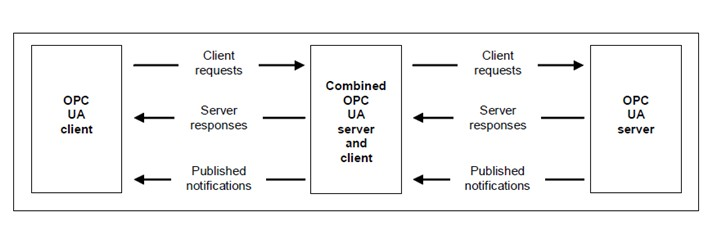
\includegraphics[width=1.00\textwidth]{cs.jpg}
		\caption[ ]{OPC UA Client Server Structure\cite{O1}}
	\label{fig:cs}
\end{figure}
Figure~\ref{fig:cs} illustrates a typical OPC UA client server architecture and also describes a combined server-client. The routine communication between client and server consists of requests from client, corresponding responses sent from server and notifications which are generated because of client’s early subscription.

\begin{figure}
	\centering
	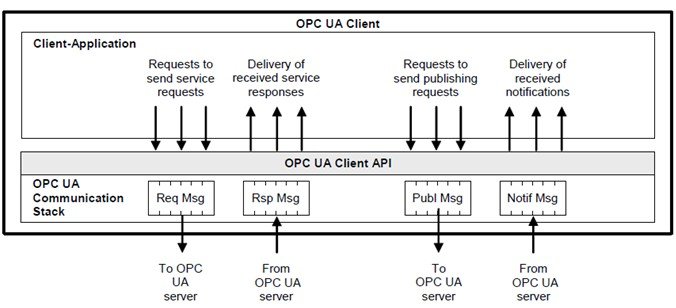
\includegraphics[width=1.1\textwidth]{client.jpg}
		\caption[ ]{OPC UA Client Structure\cite{O1}}
	\label{fig:client}
\end{figure}

Figure~\ref{fig:client} pictures one simple OPC UA client containing client application, an internal API, isolating the application code from communication stack, and a communication stack that converts API calls into messages and delivers them to OPC UA server.

\begin{figure}
	\centering
	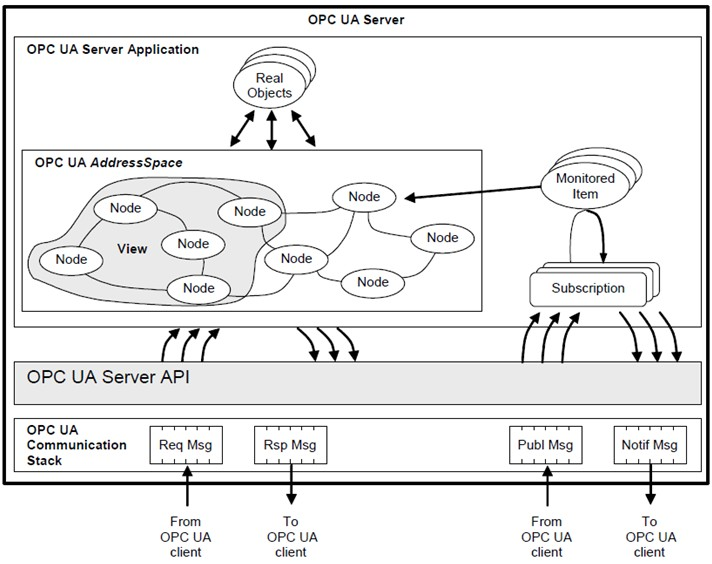
\includegraphics[width=1\textwidth]{server.jpg}
		\caption[ ]{OPC UA Server Structure\cite{O1}}
	\label{fig:server}
\end{figure}

In figure~\ref{fig:server}, one OPC UA Server structure is explained. As the aforementioned client structure, it also includes three main parts, server application, internal API and communication stack. It is worth mentioning that, real objects here are referred as physical field devices or software application that is only maintained internally. View, which is pictured as a part of address space, presents objects that can be browsed by clients

\subsection{Secure Channel and Session}
Since some data exchanged between client and server could be extreme precious and should be protected from other malicious third party, OPC UA defines a full set of security model, with which developer of system can configure the security level of the application to meet the need of reality. In the security model, authentication of client and server, authorization, integrity and confidentiality of client-server- communication, auditability and availability of services are guaranteed. Also OPC UA provides a set of countermeasures against message flooding, eavesdropping, message spoofing message alteration, message reply, server profiling, session hijacking and so on\cite{O2}.
\begin{figure}
	\centering
	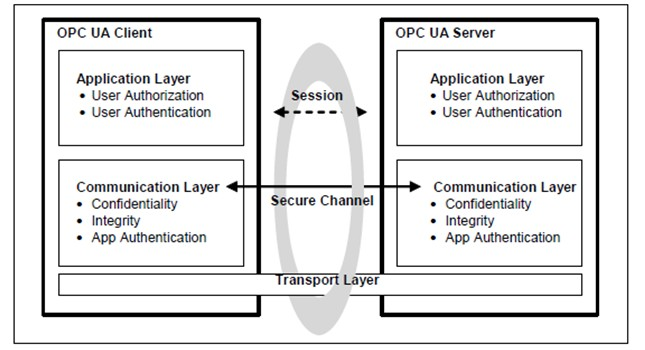
\includegraphics[width=1.1\textwidth]{opc_ua_cs_comm.jpg}
		\caption[ ]{OPC UA Client Server Communication\cite{O2}}
	\label{fig:opc_ua_cs_comm}
\end{figure}


Figure~\ref{fig:opc_ua_cs_comm} pictures the typical security communication architecture of OPC UA. As shown in~\ref{fig:opc_ua_cs_comm}, the communication between OPC UA client and server is established above a secure channel, which is active during the whole application session and in this session, the state information, such as subscriptions from client, user credentials, is maintained. The secure channel is established only after successful validation of both client and server certificates and it provides necessary mechanisms to support confidentiality, message integrity and application authentication. On top of secure channel, is an application level session between OPC UA client and server, whose responsibilities are to transmit data information and commands. This session is also in charge of managing security policies like user authorization and authentication. It should be pointed out that, even a secure channel is out of work for some reasons, the session is still valid and OPC UA client and server involved in aforementioned session can still re-establish the broken secure channel. A secure transport layer is guaranteed by encryption and signatures methods provided by platform that supports OPC UA structure.

\begin{figure}[!htb]
	\centering
	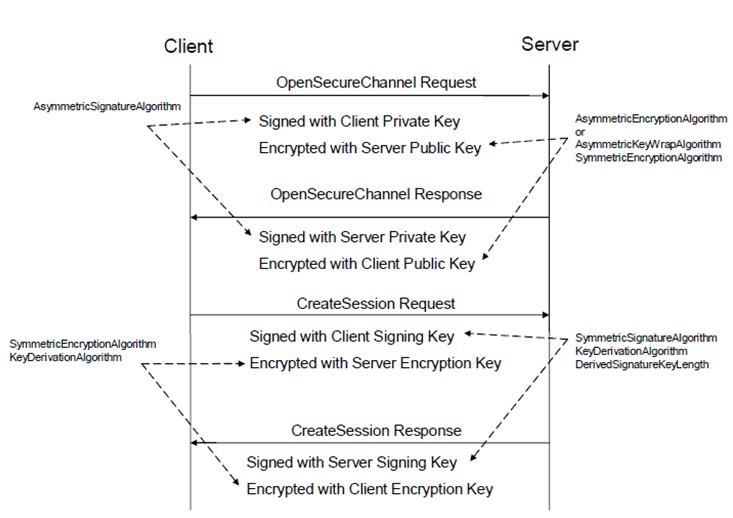
\includegraphics[width=1\textwidth]{opc_ua_shs.jpg}
		\caption[ ]{OPC UA Client Server Security Handshake\cite{O2}}
	\label{fig:opc_ua_cs_shs}
\end{figure}
\subsubsection{Security Handshake}
Security handshake as below explains with some details about how secure channel and session are established.OPC UA client initiates the first \emph{OpenSecureChannel} request and waits the response from server. Messages exchanged during the process of construction secure channel between client and server are encrypted using asymmetric encryption and signature algorithms. But some security protocols that could be applied according to OPC UA standard, are not using an asymmetric message encryption algorithm to encrypt to request/response messages. Instead, they apply AsymmetricKeyWrapAlgorithm to encrypt symmetric keys and use symmetric encryption algorithm with encrypted keys to encrypt messages. After a successful construction of secure channel, OPC UA client sends \emph{CreateSession} request and waits for server response. Messages transported during this procedure are encrypted with symmetric encryption algorithms and signed with client/server signing key.
\begin{figure}[!htb]
	\centering
	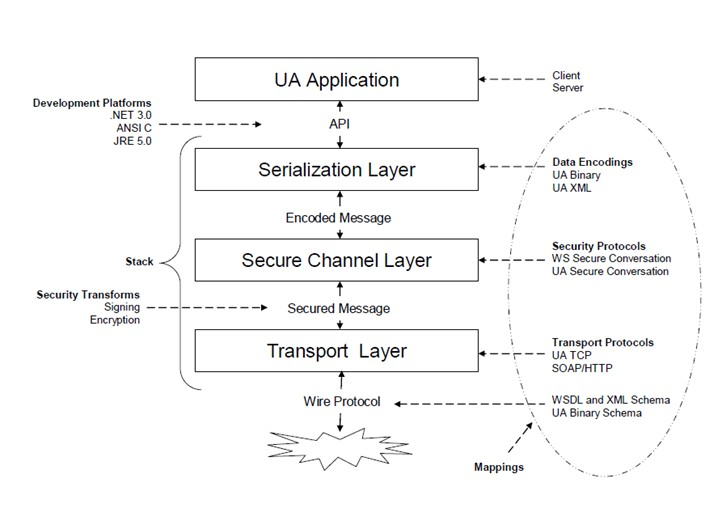
\includegraphics[width=1\textwidth]{opc_ua_commstack.jpg}
		\caption[ ]{OPC UA Client Server Communication Stack\cite{O2}}
	\label{fig:opc_ua_commstack}
\end{figure}
\subsection{OPC UA Communication stack}
As discussed in subsection 2.3, the OPC UA communication stack is a three-layer architecture: application layer, communication layer and transport layer. Even the terminologies of those layers are defined as the ones used in ISO model, but layers in OPC UA are not directly equal to layers in ISO model. Figure~\ref{fig:opc_ua_commstack} from OPC UA  6th specification\cite{O6} gives a precise overview of each layer in OPC UA communication stack model, meanwhile it demonstrates functionalities performed by each layer.

UA Application layer realizes client and server code. Serialization layer together with secure channel layer build the communication layer and their job is dividing long message into pieces referred as message chunk, encrypting each individual message chunk, not entire whole message and forwarding encrypted message chunk to transport layer. When receiving message chunk from others, OPC UA message receiver firstly verifies whether this message piece meets the security standard negotiated between OPC UA client and server. If not, this message receiver will close the secure channel. After a successful verification of all message chunks, the original OPC UA message will be reconstructed and sent to UA Application Code through API. Each secure message chunk applies the following structure described in figure~\ref{fig:opc_ua_messchunk}.

Knowing the essential parts of OPC UA communication stack, in the following subsections the establishment, re-establishment and close of communication channel are explained.
\begin{figure}
	\centering
	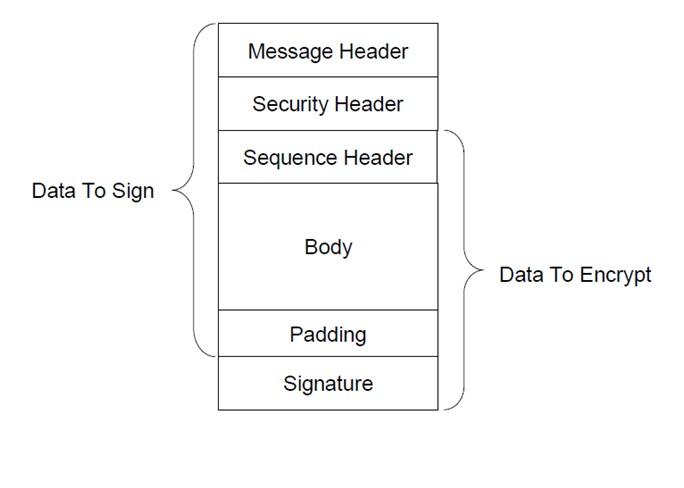
\includegraphics[width=0.75\textwidth]{opc_ua_messchunk.jpg}
		\caption[ ]{Message Chunk Structure\cite{O2}}
	\label{fig:opc_ua_messchunk}
\end{figure}

\begin{figure}[!ht]
	\centering
	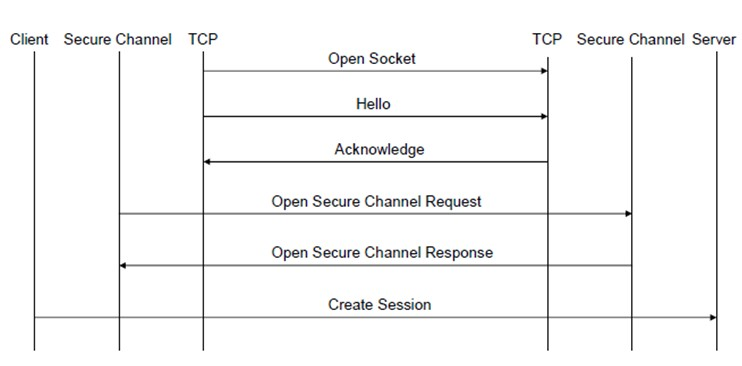
\includegraphics[width=1\textwidth]{tcp_1.jpg}
		\caption[ ]{Establish TCP/IP Connection\cite{O6}}
	\label{fig:tcp_1}
\end{figure}
\subsubsection{Establishment of communication channel}
As the first step to create TCP/IP connection, this process is always initialized by OPC UA client. OPC UA client initiates his socket and sends \emph{helloMessage}, that includes supported buffer size which specifies the message chunk size used for future communication, to the target OPC UA server. After receiving greeting message, OPC UA server answers the request for establishing TCP/IP connection with acknowledge message and reports negotiated buffer size to his own secure channel layer. Moreover during the creation of communication channel process, the greeting \emph{hallo} and answering \emph{acknowledgment} messages could only be sent once. If OPC UA client or server receives them more than one, error will be reported and corresponding communication socket will be closed. Even thought server application code does not have to work during the negotiation of secure channel process, it should provide the communication stack all his trusted certificates which help communication stack to verify the identity of the other communication partner. 
\begin{figure}[ht]
	\centering
	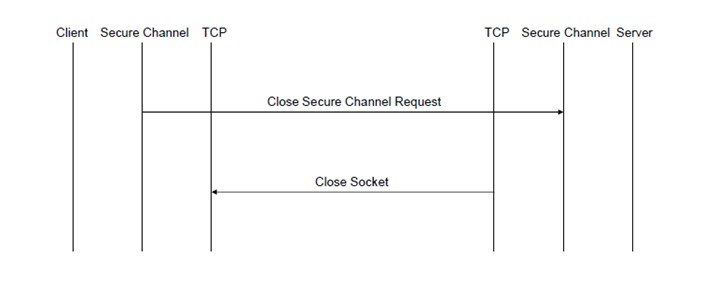
\includegraphics[width=1\textwidth]{tcp_2.jpg}
		\caption[ ]{Close TCP/IP Connection\cite{O6}}
	\label{fig:tcp_2}
\end{figure}
\subsubsection{Close TCP/IP Connection}
This process is done when OPC UA server receives \emph{CloseSecureChannel} request from OPC UA client. During this process, server releases all the resource taken by corresponding secure channel and sends none response.
\begin{figure}[ht]
	\centering
	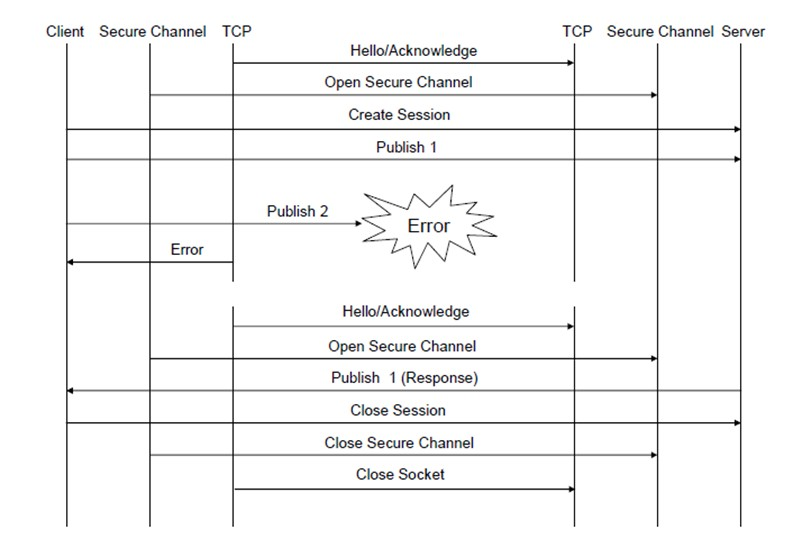
\includegraphics[width=1\textwidth]{tcp_3.jpg}
		\caption[ ]{Recover Secure Channel\cite{O6}}
	\label{fig:tcp_3}
\end{figure}

\subsubsection{Recover Secure Channel}


Whenever error occurs during TCP/IP connection between OPC UA client and server, client will try to periodically re-establish it until the session is closed or the lifetime of security token goes to an end. Also it should be pointed out that the buffer size defined by corrupt secure channel should not be changed during this error recover process.

\subsection{Historical Data}
Last but not least security feature offered by OPC Unified Architecture is auditing, which supports traceability of any behaviours occur in OPC UA system. That means any security related problem can be recorded and for future use.


\subsection{Other Competitor}
WebSphere Message Broker Message Queuing Telemetry Transport (MQTT)\cite{Ref3} is another machine to machine (M2M) communication protocol. Compared with OPC UA standard, MQTT also supports UDP protocol in the transport layer. In OPC UA, only unidirectional, client to server, communication is provided, but in MQTT server to client communication is also possible without server implements client code. Moreover the communication overhead of MQTT is in comparison with OPC UA is relative small. 


Even thought MQTT protocol supports communication environment with low bandwidth and high latency, OPC UA provides complex object model and supports more features, including historical data record, alarm, notification, complete security policies and this is reason why OPC UA is more suitable for the application scenario that handles sensitive data with complex structure and needs immediate response.


Another member from Internet of Things is Constrained Application Protocol (CoAP)\cite{Ref5} which is designed for the extreme simple electronic devices with less memory and computing power and original CoAP only runs over UDP. Compared with OPC UA, simplicity from CoAP is the advantage, but apparently it should be considered that in the implementation scenario other transport protocol could be used, like TCP, more functions and services other than pure message exchange between client and server, are requested from users.

\section{Implementation Scenario}
 \begin{figure}[!htbp]
	\centering
	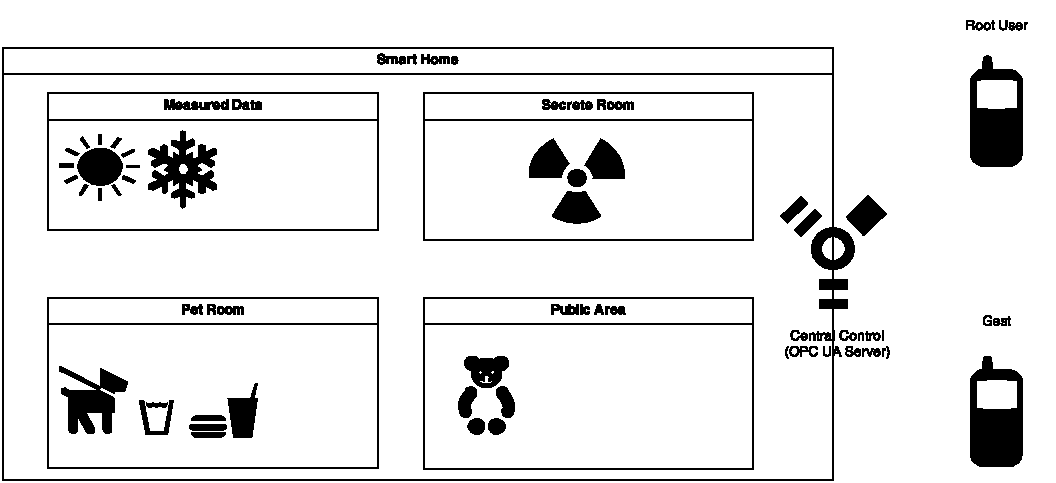
\includegraphics[width=1.2\textwidth]{SmartHome}
		\caption[ ]{Smart Home}
	\label{fig:SmartHome}
\end{figure}
Figure~\ref{fig:SmartHome} describes the basic structure and functionalities of Smart Home. Central Controller also named as OPC UA Server is in charge of monitoring predefined environment variables, for instance, home temperature, luminance and how much water the pet has, and taking corresponding behaviors, such as opening windows, turning off the heating or notifying pet owner that puppy needs water. With the help of such services a more comfortable living condition is created in an automated way. Also OPC UA Server controls access right of entering each room, which means only authenticated users with enough authority can open the door. Moreover the root user, namely the owner of this house, is capable of assigning the permission of accessing particular room to other guests. In case of when he/she is taking a vocation and pet cannot get necessary care while he/she is away. At the same time, root user won't worry about the person, who promises feeding pet, entries the forbidden room. At last, every single action taken by the OPC UA Server is recorded and is available for future use. 



In the implementation scenario, OPC UA clients are Universal Integrated Circuit Card (UICC)  based phone user and in home allocated senor. OPC UA server is a secure hard device, that is in charge of communication management with phone use and implementation of OPC UA server application code. Environment date is measured periodically by sensors and each room is locked, only the client, who is authenticated by server and holds enough authority can enter. It is assumed that handy users are in an open environment at mean while senors in home have a relative secure wifi connection with OPC UA server. Smart card that is applied in this scenario also acts as security token for OPC UA client, which contains credential information like encryption keys. certificates and digital signature. Moreover the communication stack is developed and integrated on smart card, which means without corresponding UICC card, OPC UA client and server are not able to appropriately finish their work.
 \begin{figure}[ht]
	\centering
	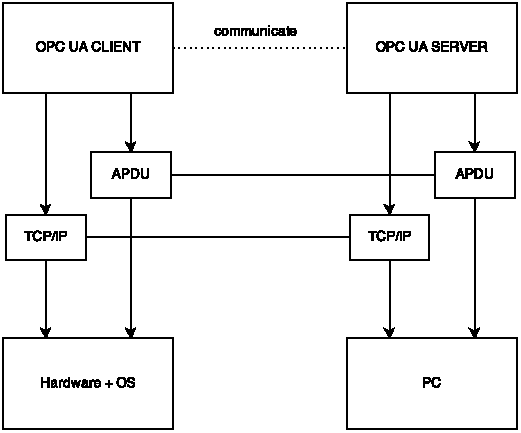
\includegraphics[width=1\textwidth]{softwareStructure}
		\caption[ ]{OPC UA Client Server Based On TCP/IP or APDU}
	\label{fig:softwareStructure}
\end{figure}

Figure~\ref{fig:softwareStructure}, describes possible software structure of aforementioned OPC UA client server structure. With different chip card, OPC UA client application is able to communicate with server using Application Protocol Data Unit(APDU) and Short Message Service(SMS), which is a more nature and traditional way to exchange date with chip card, or TCP/IP based web service when components from Global Platform\footnote{Global Platform is a cross industry, non-profit organization that develops and publishes standard in secure chip technology.} is applied or newly released Javacard 3 is used.  

\subsection {Software Structure}
According to the above-mentioned application scenario, UA application client and server code will be written using Java, deployed as Handy application, OTA server respectively. 
Basic functions as following are provided:
 \begin{itemize}
  \item subscription/publishing environment data
  \item secure message exchange
  \item authority management
  \item historical data management
  \item running client's command
\end{itemize}
Communication stack is develop on UICC smart card realizing secure channel and session management, transporting data to message chunk receiver using Tcp/IP connections. An internal API translates OPC UA application instructions in to Application Protocol Data Unity (APDU) messagse and forwards them to smart card, which is in charge of user authentication and processing secure messaging between card application and chip card pair. 
\subsubsection{Smart Card Security}
As explained, smart cards are widely used in applications that require strong protection. With sophisticated communication protocol using Application Protocol Data Units, smart card and Card Accepting Device(CAD) are able to process secure message exchange and bidirectional authentication. Moreover sensitive data like certificates, encryption keys are stored on card along with other precious user information and this data is extreme difficult to be altered by third party .Most of time smart card also acts as secure token and can process cryptographic algorithms on hardware. Nowadays, smart card supports symmetric key algorithms like DES, triple DES; standard public key cryptography for instance RSA, hash functions such as commonly SHA-1\cite{handbuch}. More powerful microprocessor on chip card is, the speed performance is better.  

Moreover thanks to self-containment structure, smart card itself does not dependent on other external resources, which could be extreme vulnerable to potential secure attack, and therefore provides a better hardware security and OS security.

 \begin{figure}
	\centering
	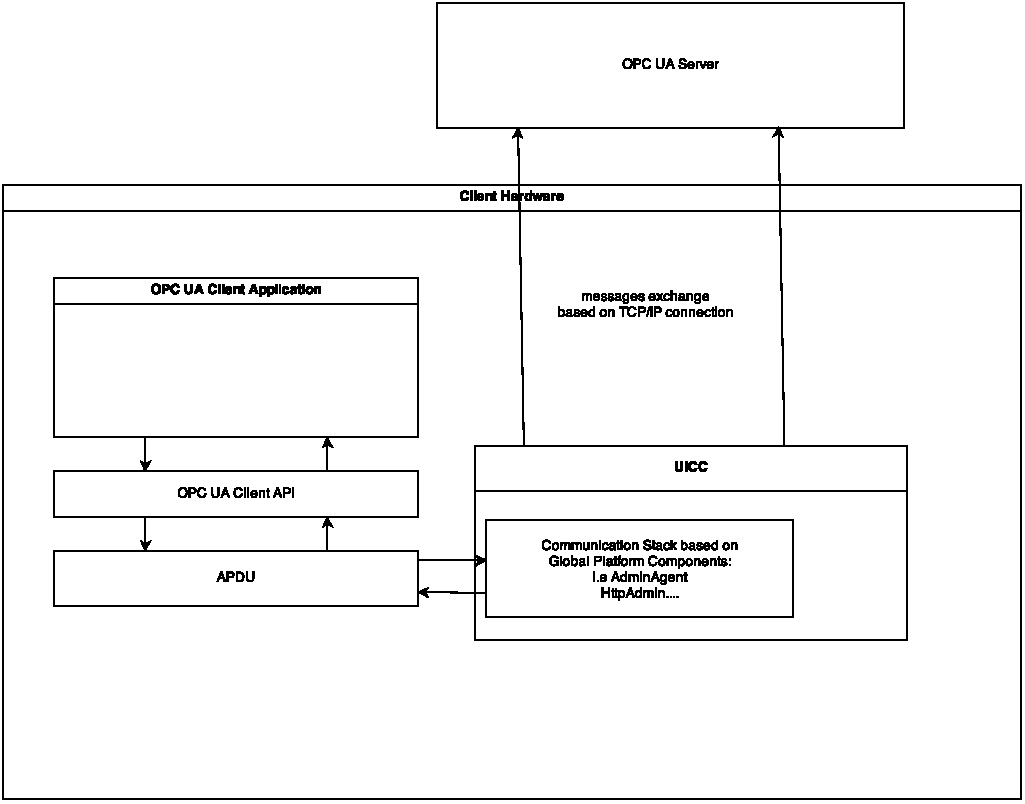
\includegraphics[width=1.0\textwidth]{clientStructure}
		\caption[ ]{Client Structure}
	\label{fig:clientStructure}
\end{figure}
\subsubsection{Client Structure}
As described in figure~\ref{fig:clientStructure}, the OPC UA client consists of client application code that realizes client application level functions, OPC UA client API that translates client application instructions into APDU and forwards APDU to UICC smart card. The Communication stack is developed and integrated with UICC card, which is in charge of creation and management TCP/IP connection, secure channel between client and server. This communication stack is based on card OS components provided by Global Platform. 
\begin{figure}
	\centering
	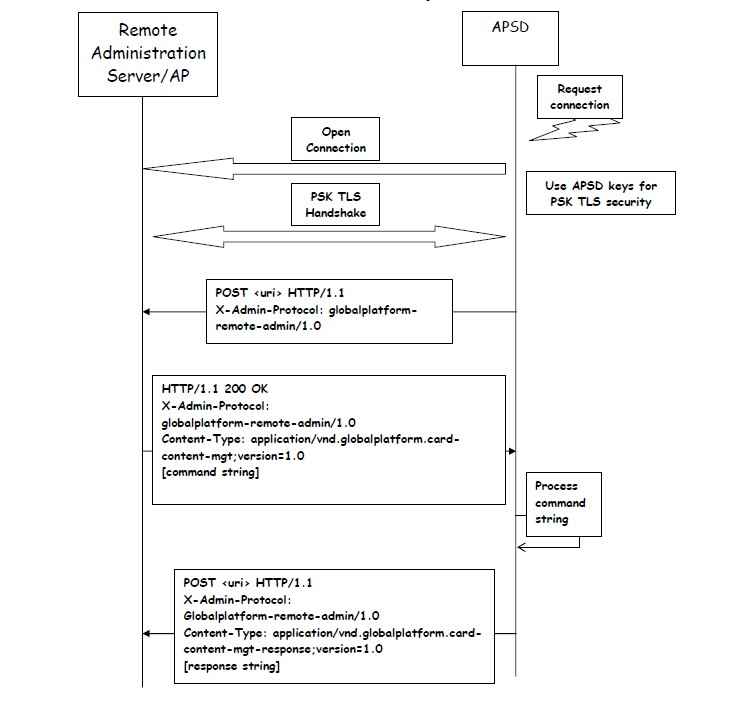
\includegraphics[width=1.2\textwidth]{apsd.jpg}
		\caption[ ]{Communication Flow between an AP and corresponding APSD\cite{ramGP}}
	\label{fig:apsd}
\end{figure}
Global Platform provides and defines communication flow between an application provider and smart card, allows information exchanged between a remote entity and a card. The on card component, which is responsible for connection creation with the remote entity, is called Security Domain. And the remote entity also is referred as Remote Administration Server. With those concepts, smart card with Security Domain can act as HTTP client and is capable of packing APDU formate information into HTTP POST message. At the same time, the Remote Administration Server also is a HTTP server, which can send HTTP message including APDU format information to its client.\cite{ramGP}
 
Figure~\ref{fig:apsd} illustrates a typical communication flow between administration server and corresponding security domain on smart card. As can be seen, the request for open communication is alway initialized by security domain, which is also the phone user. After a successful creation of secure handshake, the remote administration server and security domain is able to using HTTP message to exchange command and response strings, which include APDU instructions from OPC UA client and server.

\begin{figure}
	\centering
	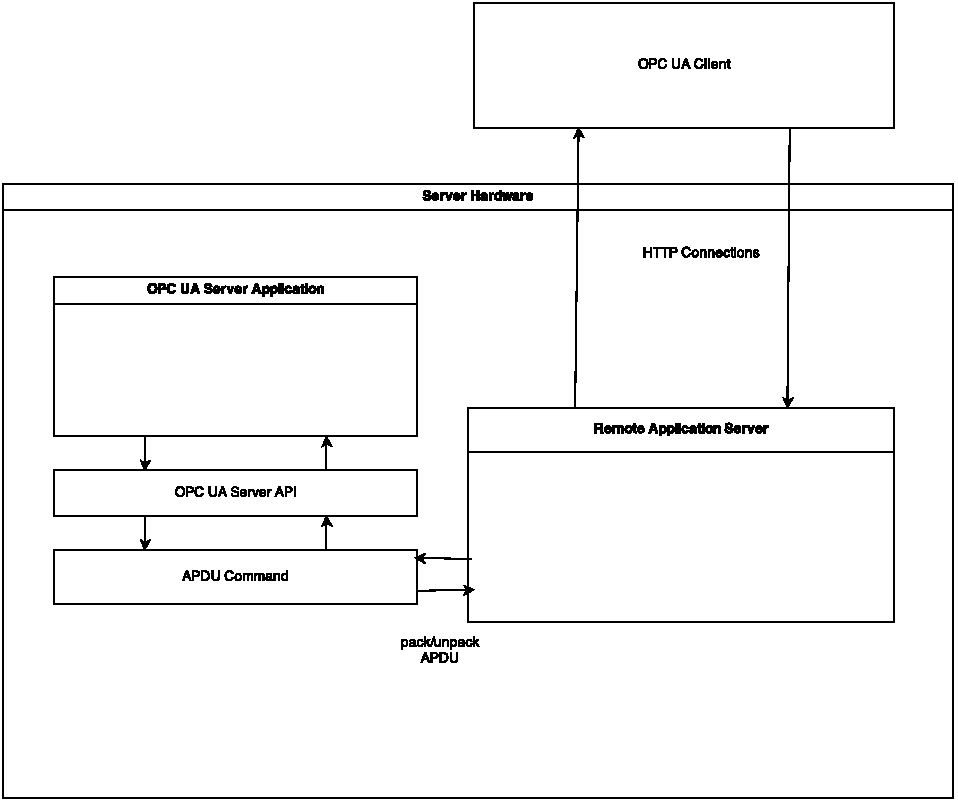
\includegraphics[width=1.0\textwidth]{serverStructure}
		\caption[ ]{Server Structure}
	\label{fig:serverStructure}
\end{figure}
\subsubsection{Server Structure}
The server structure for Smart Home is pictured as figure~\ref{fig:serverStructure} and it consists of an OPC UA server application that implements smart home server services, a remote application server, which realizes server side communication stack, together with on card embedded security domain manages HTTP connections, secure channel construction as well as user authentication. 
\section{Time Lines}
 \begin{itemize}
  \item read paper, documentation, reference
  \item design dummy client/server application code 
  \item analyze and design communication stack that fits UICC card and meets OPC UA standard 
  \item combine application code and communication stack
  \item analyze design and apply secure protocols. 
  \item debugging/performance analysis
\end{itemize}

\bibliographystyle{splncs}
\bibliography{opc_ua}
\end{document}
